\newpage
\section{Amplificador VFA - CFA con red de compensación}

\hspace{1mm} Se procede a añadir una red de compensación cero-polo a la configuración anterior, con el propósito específico de cancelar el polo ubicado en $5.06~MHz$ del amplificador VFA.

\begin{figure}[!h]
    \centering
    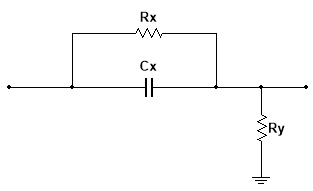
\includegraphics[width=0.5\linewidth]{figuras/12. Red de compensacion RC.png}
    \caption{Red de Compensación RC.}
\end{figure}

\hspace{1mm} En esta representación gráfica, se destacan los elementos clave de la red de compensación, como la ubicación del cero y del polo diseñados para contrarrestar el efecto del polo $f_2 = 5.06~MHz$.



\subsection{Análisis teórico}
\hspace{1mm} La red de compensación cuenta con la siguiente función transferencia 

\begin{equation}
    A_c(s) = \frac{R_y}{R_x + R_y} \cdot \frac{1 + sC_x R_x}{1 + sC_x (R_x // R_y)}
\end{equation}

\hspace{1mm} donde se han definido las siguientes notaciones:

\begin{itemize}[itemsep=1pt]
    \item $k_{comp}=\frac{R_y}{R_x + R_y}$
    \item $ \omega_{pcomp} =  \frac{1 }{1 + sC_x (R_x // R_y)}$
    \item $\omega_{zcomp} = \frac{1 }{ C_xR_x}$
\end{itemize}

\hspace{1mm} Dado que el cero del compensador debe cancelar el polo producido por $f_2$, se tendrá

\begin{equation}
    \Longrightarrow \omega_{zcomp} = \omega_2 = 2\pi \cdot 5.06~Mrps
\end{equation}

\hspace{1mm} Como se solicitó en la consigna, el polo de compensación se ubicará una octava por encima de este cero, resultando entonces:

\begin{equation}
    \omega _{pcomp} = 2\cdot\omega _{zcomp} = 2\pi \cdot 10.12~Mrps 
\end{equation}
\\
\hspace{1mm} Con estos valores deducidos, es posible calcular la ganancia del compensador

\begin{equation}
    k_{comp} = \frac{\omega_{zcomp}}{\omega _{pcomp}} = \frac{2\pi \cdot 5.06~Mrps}{2\pi \cdot 10.12~Mrps}
\end{equation}

\begin{equation}
    \boxed{
    k_{comp} = 0.5
    }
\end{equation}

\hspace{1mm} Recordando que

\begin{equation}
    k_{comp} = \frac{R_y}{R_x + R_y}  \Longrightarrow  ~ \frac{R_y}{R_x + R_y} = 0.5
\end{equation}

\hspace{1mm} Despejando para obtener la relación entre las resistencias
\begin{align}
    \frac{R_y}{R_x + R_y} &= \frac{1}{2}        \\
                     2R_y &= R_x + R_y           \\
                        2 &= \frac{R_x}{R_y} + 1
\end{align}

\begin{equation}
    \boxed{
    1 = \frac{R_x}{R_y}
    }
\end{equation}

\hspace{1mm} Considerando valores normales 

\begin{equation}
    \boxed{
    R_x = R_y = 1~k\Omega
    }
\end{equation}

\hspace{1mm} Obtenido el valor de las resistencias, es posible calcular el valor del capacitor $C_x$, despejando de la ecuación del cero 

\begin{equation}
    \begin{aligned}
              \omega_{zcomp} &= \frac{1}{C_x R_x}                     \\
        \Longrightarrow C_x &= \frac{1}{\omega_{zcomp} \cdot {R_x}}  \\
                        C_x &= \frac{1}{2\pi \cdot 5.06~Mrps \cdot 1~k\Omega}
    \end{aligned}
\end{equation}

\begin{equation}
    \boxed{
    C_x = 31~pF
    }
\end{equation}


\hspace{1mm} Al agregar el compensador, se obtiene la siguiente función de transferencia del lazo de realimentación:

\begin{equation}
    \begin{aligned}
        T(s) &= -A_d(s) \cdot A_c(s) \cdot A_{vf2} (s)\\
             &= - \frac{k\cdot A_d(0)}{\left(1+\frac{s}{\omega_1}\right)\left(1+\frac{s}{\omega_2}\right)} \cdot k_{comp} \frac{\left(1 + \frac{s}{\omega_{zcomp}}\right)}{\left(1+\frac{s}{\omega_{pcomp}}\right)} \cdot A_{vf2}(s)
    \end{aligned}
\end{equation}


\hspace{1mm} donde:

\begin{itemize}[itemsep=1pt]
    \item $k:$ realimentación del VFA.
    \item $A_d(0):$ ganancia del VFA.
    \item $A_{vf2}:$ función de transferencia del CFA.
    \item $ \omega_1 , \omega_2 :$ los polos del VFA.
\end{itemize}

\hspace{1mm} Se observa que el valor de $k_{comp}$ induce una atenuación en la función de transferencia, y por ende, en la ganancia. Por ello, es necesario ajustar la ganancia a lazo cerrado del CFA, teniendo en cuenta que $ k_{comp} = 0.5 $:

\begin{equation}
    A_{vf2 comp} (s) = 2\cdot A_{vf2}(s)
\end{equation}

\hspace{1mm} Esta relación garantiza que la atenuación provocada por $k_{comp}$ se compense adecuadamente en la ganancia a lazo cerrado del Compensador de Fase Avanzada (CFA), asegurando así un rendimiento equilibrado del sistema. Recordando que $A_{vf2}$ es:

\begin{equation}
    A_{vf2} = 1 + \frac{R_2}{R_1}
\end{equation}

\hspace{1mm} Reemplazando se obtiene.

\begin{equation}
    \begin{aligned}
        A_{vf2 comp} (s) &= 2 \left( 1 + \frac{R_2}{R_1} \right)\\
             &= 2 \cdot 20
    \end{aligned}
\end{equation}

\begin{equation}
    \boxed{
    A_{vf2 comp} (s) = 40
    }
\end{equation}

\hspace{1mm} Dado que el polo del CFA permanece invariable con respecto al caso anterior, el valor de $R_2$ continúa siendo 

\begin{equation}
    \boxed{
    R_2 = 850~\Omega
    }
\end{equation}

\hspace{1mm} Por su parte, $R_1$ se obtiene de:

\begin{equation}
    \begin{aligned}
        \frac{R_2}{R_1} &= 40 - 1 \\
    \Longrightarrow R_1 &= \frac{850~\Omega}{39}
    \end{aligned}
\end{equation}

\begin{equation}
    \boxed{
    R_1 = 21.8~\Omega
    }
\end{equation}

\hspace{1mm} El margen de fase ( $M\varphi$ ) se determina como la diferencia entre $180^o$ y la suma de los ángulos de las funciones de ganancia a lazo cerrado del Amplificador (VFA1), la función de ganancia a lazo cerrado del Compensador de Fase Avanzada (CFA), y el ángulo de la función de transferencia del Compensador. En este caso:

\begin{align}
   M\varphi &= 180^o - arctg \left(  \frac{f_g}{f_{VFA1}}\right) - arctg \left( \frac{f_g}{f_{p comp}} \right) - arctg \left( \frac{f_g}{f_{CFA}} \right) \label{eq:primera} \\
   \nonumber
   \\ 
   &= 180^o - arctg \left(  \frac{2~MHz}{10~Hz}\right) - arctg \left( \frac{2~MHz}{10.12~MHz} \right) - arctg \left( \frac{2~MHz}{39~MHz} \right) \label{eq:primera} \\
   \nonumber
   \\ 
    &= 180^o - 90^o - 11.18^o - 2.936^o
\end{align}


\begin{equation}
    \boxed{
    M\varphi = 75.885^o
    }
\end{equation}

\hspace{1mm} Finalmente, el ancho de banda potencial permanece inalterado en relación con el caso anterior, manteniéndose en $2~MHz$. La frecuencia del polo de la función de transferencia a lazo cerrado se calcula aplicando el producto ganancia por ancho de banda:

\begin{equation}
    A_{vf} (0) \cdot f_g = A_{vf}(-3~dB) \cdot f_p
\end{equation}


\hspace{1mm} Despejando $f_p$

\begin{align}
   f_p &= \frac{A_{vf} (0) \cdot f_g}{A_{vf}(-3~dB)} \label{eq:primera} \\
   \nonumber
   \\ 
       &= \frac{10.2~MHz}{7.079}
\end{align}

\begin{equation}
    \boxed{
    f_p = 2.825~MHz
    }
\end{equation}

\hspace{1mm} Por lo tanto, el ancho de banda a $-3~dB$ resulta igual a la frecuencia del polo, es decir, $2.825~MHz$.




\subsection{Simulaciones}
Al igual que en el caso anterior, se procedió a simular el circuito, pero esta vez añadiendo la red de compensación, resultando el circuito:

\begin{figure}[H]
    \centering
    
\includegraphics[width=0.9\textwidth]{figuras/Circuito3.png}
    \caption{Circuito VFA - CFA con red de compensación}
\end{figure}

Se graficaron tanto a señal de entrada como la de salida, obteniendo una ganancia de:
\begin{equation*}
    G = \frac{V_{out}}{V_{in}}=\frac{97.36~mV}{10~mv}
\end{equation*}
\begin{equation*}
    \boxed{G = 9.736}
\end{equation*}

El error en este caso aumentó ligeramente a $2.64\%$.

\begin{figure}[H]
    \centering
    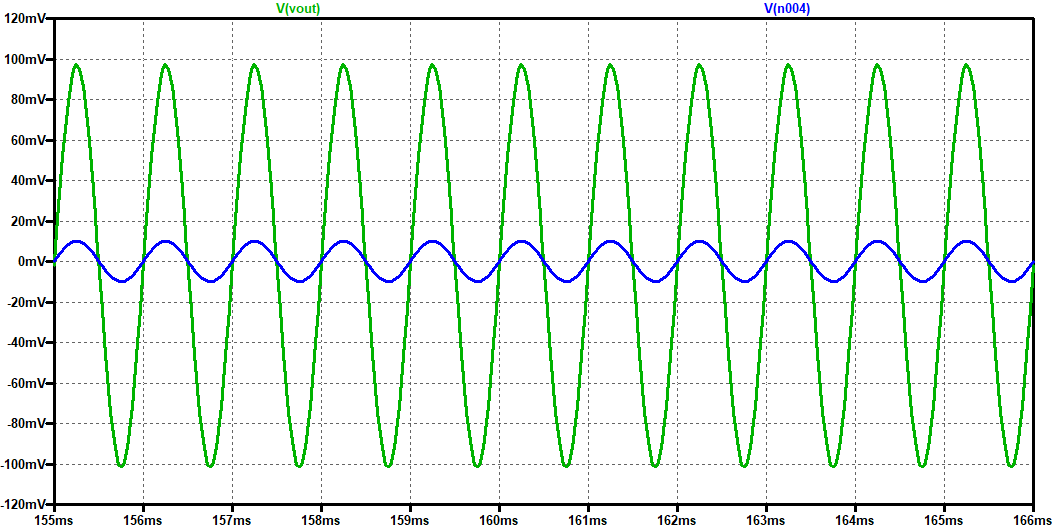
\includegraphics[width=0.9\textwidth]{figuras/Ganancia_c3.png}
    \caption{Ganancia del circuito VFA - CFA con red de compensación}
\end{figure}

Finalmente, se obtuvo el diagrama de Bode, el cual mostraba una ganancia de $20~dB$. En este caso, la caída de $-3~dB$ se presentó a una frecuencia de $2.5~dB$, lo que implicó un error de $24.38\%$.

\begin{figure}[H]
    \centering
    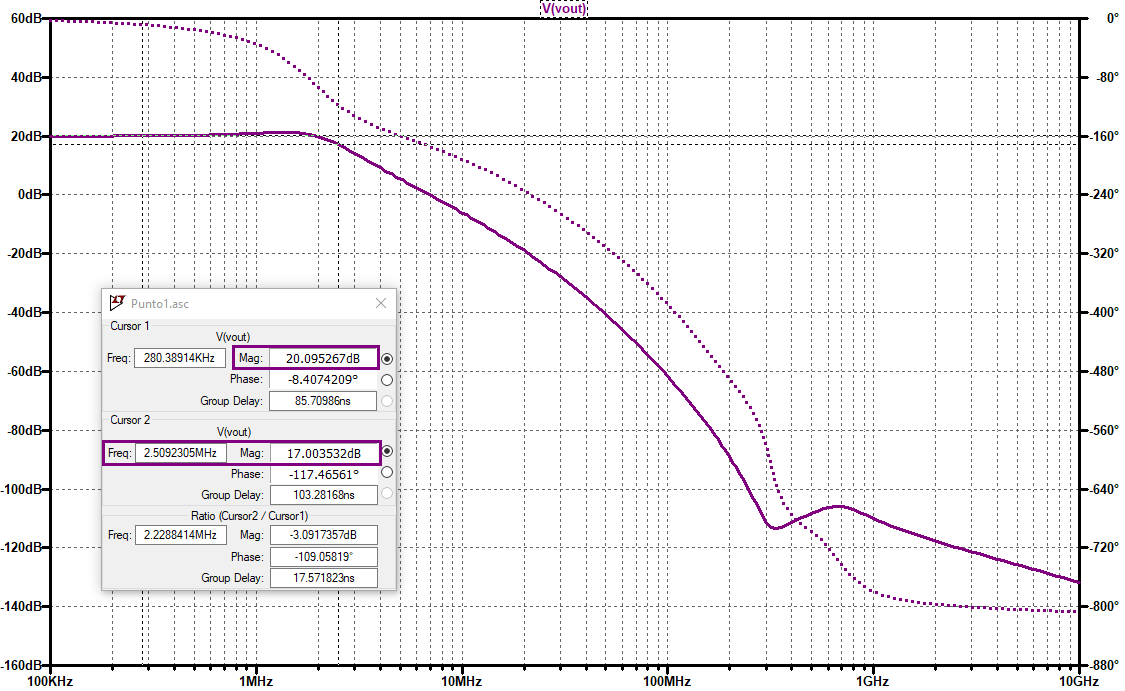
\includegraphics[width=0.9\textwidth]{figuras/Bode_c3.png}
    \caption{Diagrama de Bode del circuito VFA - CFA con red de compensación}
\end{figure}


\subsection{Conclusión}
En este apartado se realizaron todos los cálculos de las resistencias y el capacitor que comprendían la red de compensación solicitada. Esta red permitió cancelar eficazmente el efecto del polo adicional en la frecuencia de $5.06~MHz$ del amplificador VFA-CFA, ajustando así la respuesta del sistema y mejorando mejorar su estabilidad. 

\bigskip
La ganancia del sistema en este caso presentó un error de $2.64\%$, ligeramente mayor al caso anterior donde se obtuvo una discrepancia de $2.48\%$. Por su parte, en la respuesta en frecuencia se calculó un error de $24.38\%$, en este caso ligeramente menor comparado con los $26.87\%$. Por lo tanto, posible compensar el sistema eficazmente sin introducir errores adicionales.
